\documentclass[10pt,a4paper,twoside]{report}
\usepackage[utf8]{inputenc}
%Algemene documentinstellingen als dubbelzijdig, codering, rapportsoort etc.

\usepackage[dutch]{babel}
\usepackage[backend=biber,style=apa,sorting=nty,natbib]{biblatex}
\addbibresource{bibliografie.bib}
\DeclareLanguageMapping{dutch}{dutch-apa}
%APA-richtlijnen en taalinstellingen

\usepackage{afterpage}
\newcommand\blankpage{
    \null
    \thispagestyle{empty}
    \newpage}
%Code om blanke pagina's in te voegen
%Code is \afterpage{\blankpage}

\usepackage{graphicx}
\graphicspath{ {./Images/} }
%Om figuren in te voegen

\usepackage{fancyhdr} %Voet- en kopteksten
\usepackage{csquotes} %Quotes die Babel respecteren
\usepackage{lastpage} %Variabele voor paginanummering
\usepackage{booktabs} %Tabeloptimalisatie
\usepackage{pdfpages} %Samenvoegen van PDF's 
\usepackage{lipsum} %Lorem ipsum
\usepackage[pages=some]{background} %Achtergrondafbeeldingen bij voorwoord

\usepackage[linktoc=all]{hyperref}
\hypersetup{
    colorlinks=true,
    linkcolor=black,
    filecolor=cyan,
    urlcolor=cyan,
    citecolor=black,
    breaklinks=true,
    bookmarksopen=true}

%Links naar websites, bronnen, inhoudsopgave, pagina's etc.

\def\titel{Afstudeerwerkplan Seafood Connection}
\def\ondertitel{Convergerende uitwerking van de opdrachtformulering en -omgeving als hulpmiddel \\
voor de afstudeeropdracht bij Seafood Connection B.V. te Urk}
\def\auteur{Gerrit Post}
\def\studentklas{S1071236 --- AC4V}
\def\mailstudent{S1071236@student.windesheim.nl}
\def\telstudent{+31 642 678 172}
\def\school{Hogeschool Windesheim}
\def\domein{Accountancy, BMR}
\def\mailschool{a.vanden.brandhof@windesheim.nl}
\def\organisatie{Seafood Connection B.V.}
\def\mailorganisatie{info@seafoodconnection.nl}
\def\telorganisatie{+31 527 687 066}
\def\docent{Drs. A. Dannenberg RA}
\def\begeleidereen{L. Brouwer, MSc.}
\def\begeleidertwee{J.J. Molenaar, MSc.}
\def\datum{21 september 2018} %Alle variabelen in het document als titel, datum etc.

\title{\titel}
\author{\auteur}
\date{\datum}
%Documenteigenschappen worden hier gekopieerd uit Definities.tex

%EIND VAN PREAMBLE


\begin{document}
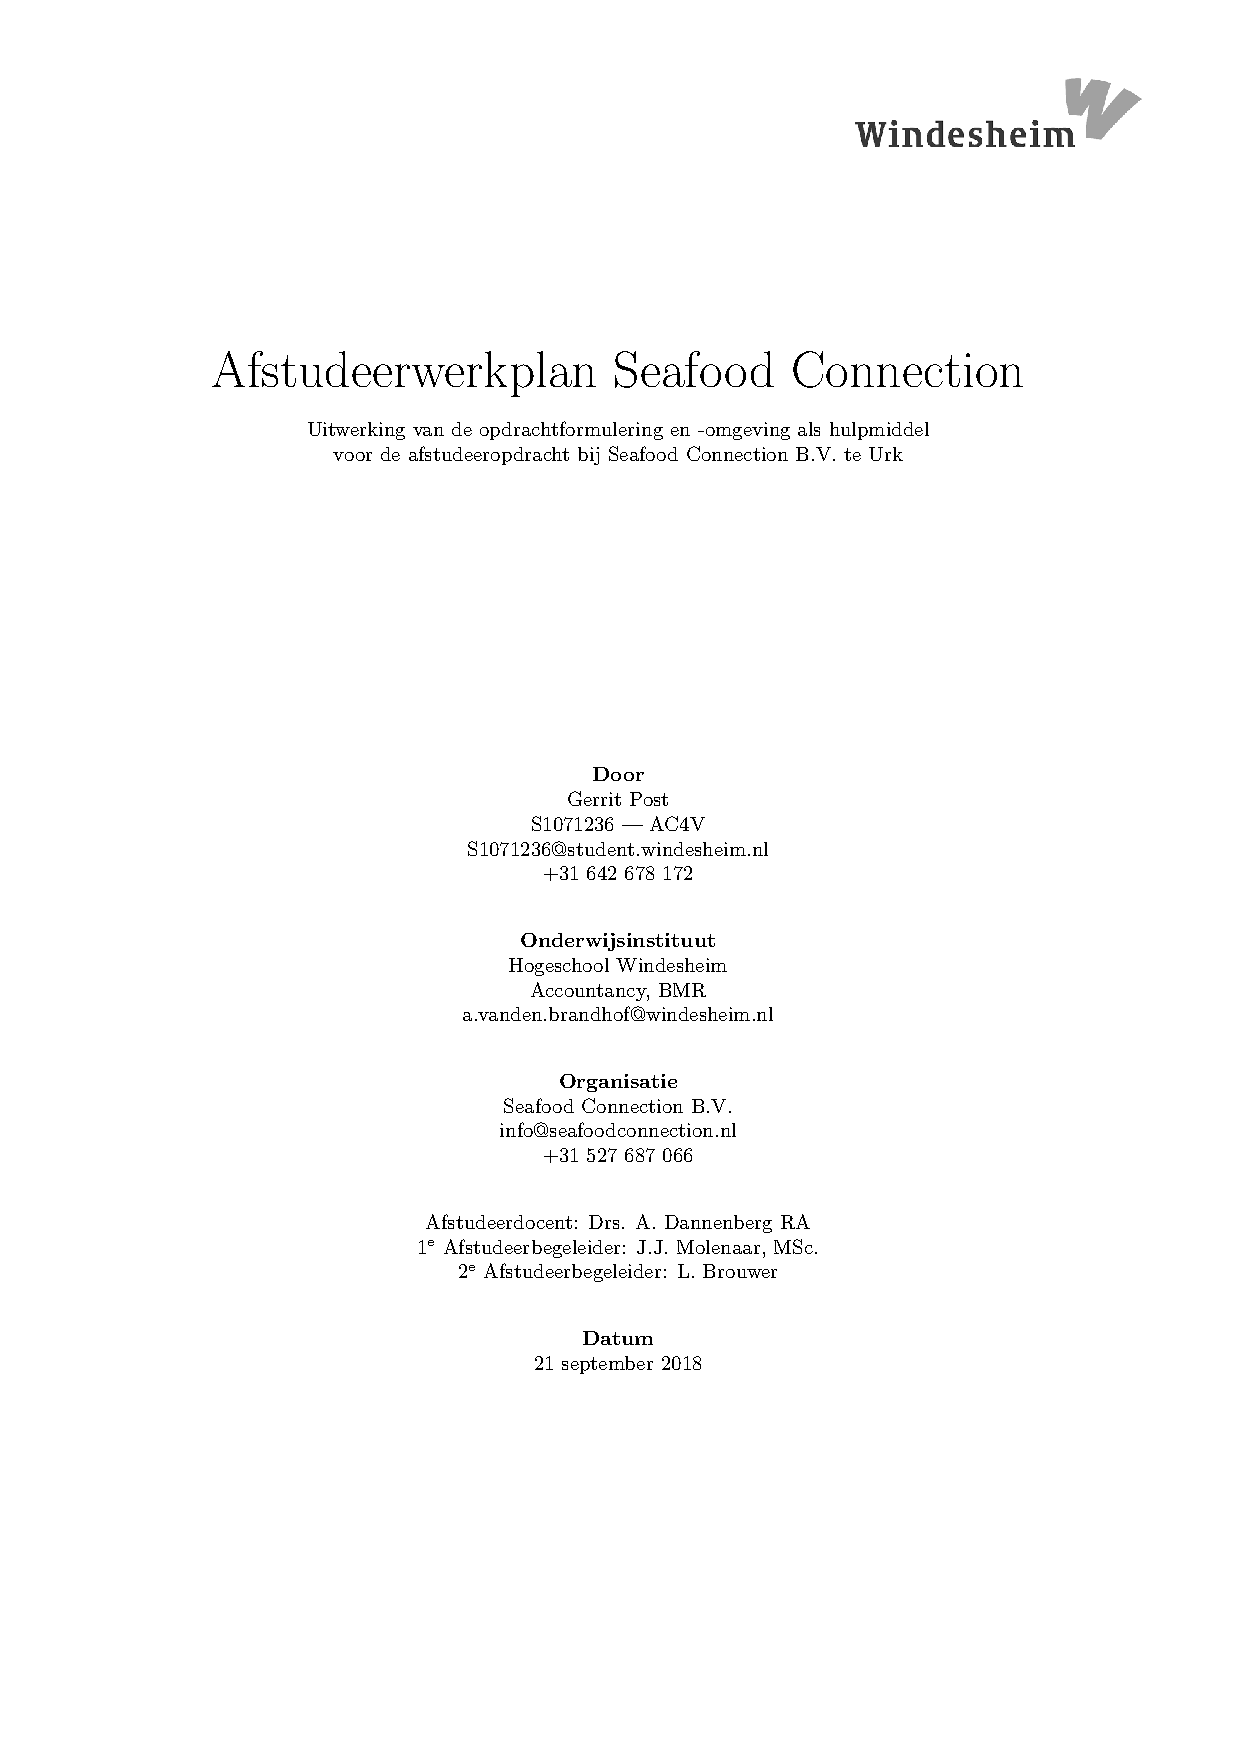
\includepdf{Titelpagina/titelpagina.pdf}
\afterpage{\blankpage}
\backgroundsetup{contents=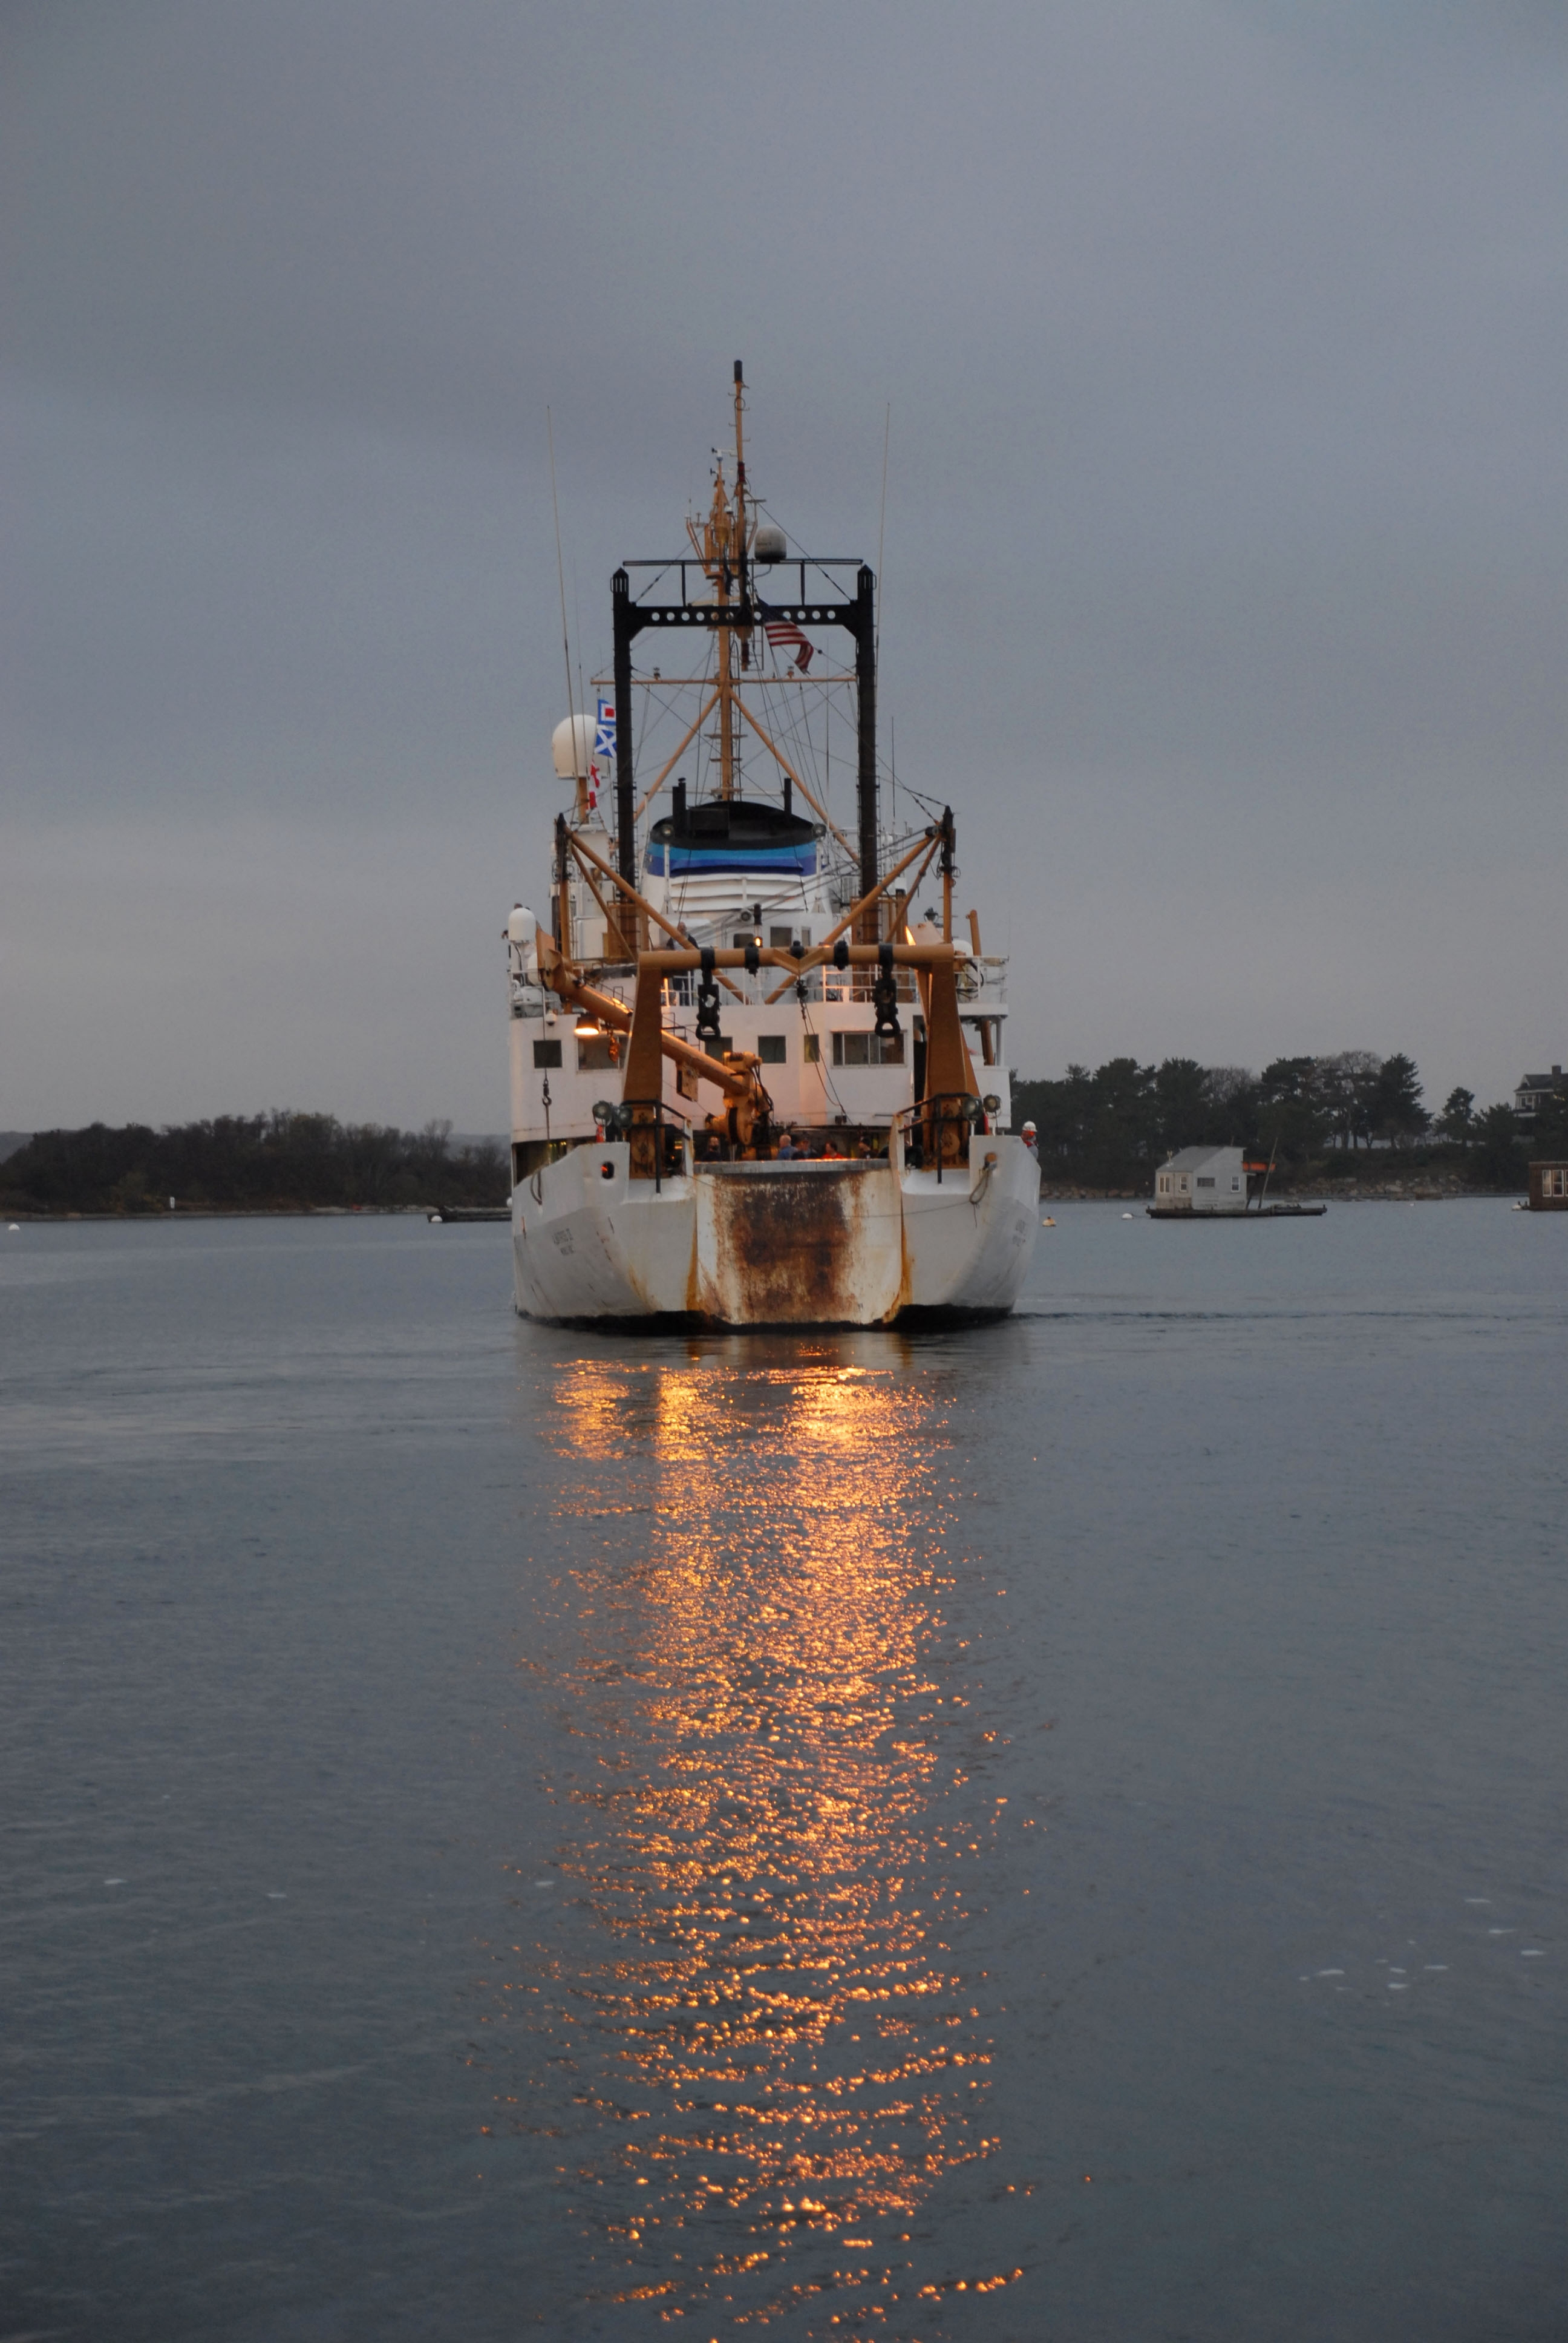
\includegraphics{3},angle=0,scale=1,opacity=1}
\BgThispage
%Titelblad wordt geïmporteerd als PDF want die is oneside en dit document twoside, zie eerste regel
%Na titelblad een lege pagina zodat er niets op de achterkant staat als hij dubbelzijdig wordt geprint

\chapter*{Voorwoord}
\thispagestyle{empty}
\backgroundsetup{contents=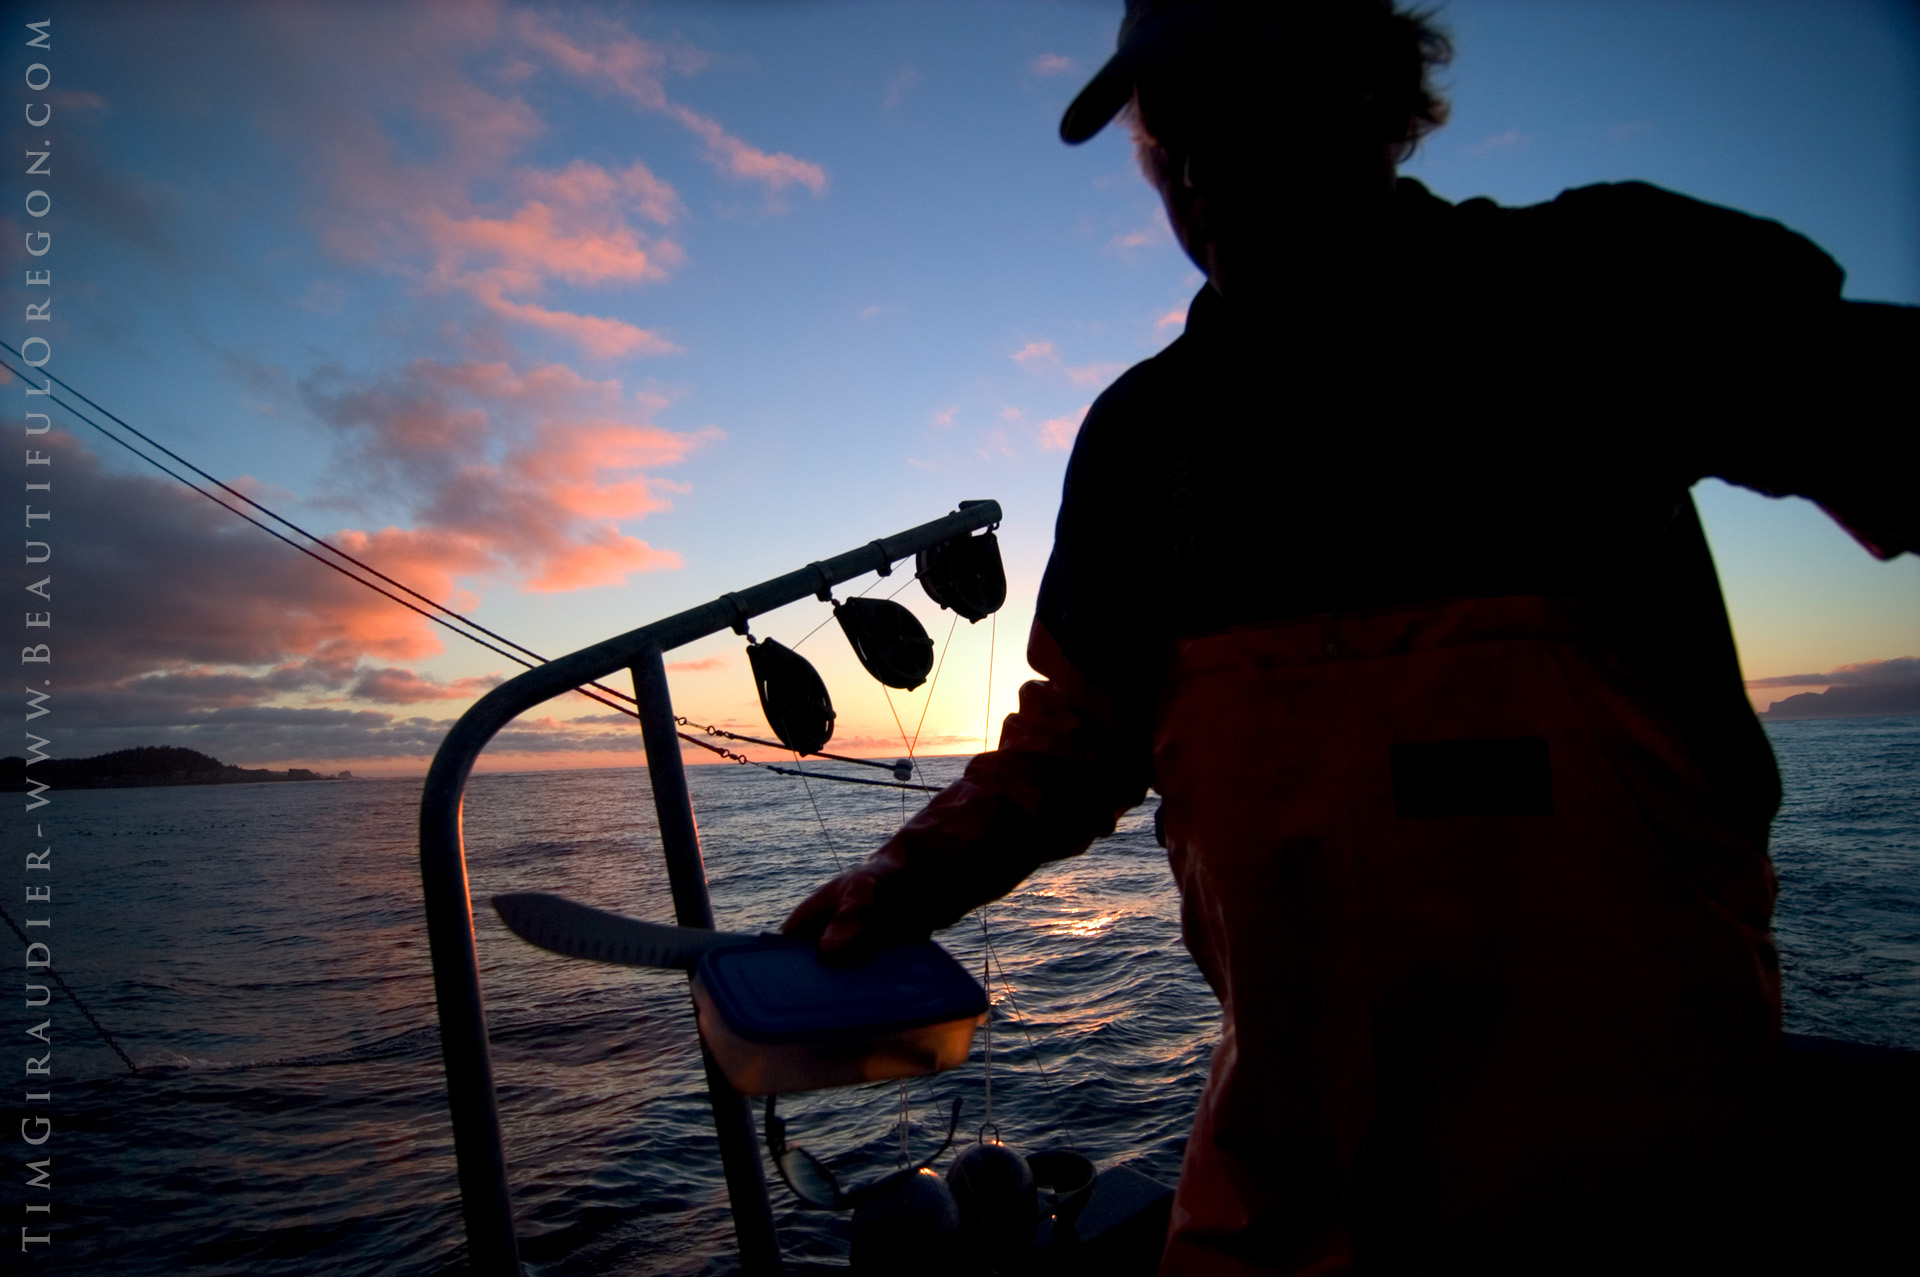
\includegraphics{7},angle=0,scale=0.68,opacity=0.65,hshift=150}
\BgThispage
\lipsum[1]
%\vfill
%{\footnotesize\textsf{\textcolor{white}{Giraudier, Tim (2018). Cross Sound, Alaska.}}}

%Voorwoord met achtergrondafbeelding

\chapter*{Samenvatting}
\thispagestyle{empty}
\lipsum[1-4]

\setcounter{page}{4} %Door importeren van PDF klopt paginanummer niet, hierbij gecorrigeerd
\tableofcontents
\thispagestyle{empty}

\chapter*{Inleiding}
\addcontentsline{toc}{chapter}{Inleiding} %Ongenummerde chapters komen niet in de ToC, met deze code wel
Ten behoeve van het definiëren en verkennen van de uit te voeren opdracht in het kader van het afstudeertraject, wordt in dit rapport met een brede blik gekeken naar de uitvoering hier van. In samenwerking met de finance afdeling van Seafood Connection wordt georiënteerd op de opdrachtformulering en wordt ook de opdrachtomgeving bekeken aan de hand van een bondige bedrijfsverkenning. Deze divergerende blik zal helpen om de opdracht in een zo’n breed mogelijke zin te bekijken. Een stapje terug doen voor perspectief als het ware.

\chapter{Inventarisatie en aanleiding}
\section{Probleemomschrijving en -aanleiding}
De AOIB bij Seafood Connection (SFC) is in lichte mate verouderd, concreet betekent dit dat sinds de laatste update er nieuwe afdelingen zijn ontstaan, er nieuwe functies zijn gecreëerd of zijn veranderd, en dat het organogram veranderd is. Het bedrijf is sinds de laatste update haast verdubbeld qua omzet en personeel, om deze reden ziet het management graag een update van deze AOIB. 

Daarnaast is er nog niet een beleid omtrent de treasury. Om deze reden is er een nood aan een vastgelegde treasury statuut waarin de bevoegdheden, verantwoordelijkheden, toezichtmaatregelen, de sturing, en beheersing geformuleerd worden ten aanzien van financiële vermogenswaarden, financiële geldstromen, financiële posities en de hieraan verbonden risico’s. \citep{ede,handreiking}

Samenvattend worden de huidige bestaande organisatorische maatregelen en processen in kaart gebracht. Daarnaast is het management van SFC bewust dat er op een navolgbare en verantwoordelijke manier omgegaan moet worden met financiële middelen; immers handelt het bedrijf met een uitputbare hoeveelheid vreemde valuta en is er een hoge mate van liquiditeit vereist om het bestaan van het bedrijf in de toekomst te kunnen garanderen.

\section{Betrokken partijen}
De betrokken partijen bij dit probleem zijn echter niet alleen de leden van het management. De inrichting en het vormgeven van de organisatie heeft direct invloed op alle bedrijfsprocessen en de werknemers werkzaam in de waardeketen. Het is voor de beheersing van de processen belangrijk dat de afstudeerstagiair gesprekken aangaat met niet alleen de afdelingshoofden, maar ook de assistenten die direct onder leiding van het middenmanagement staan. Bij de dagelijkse werkzaamheden wordt niet bewust nagedacht over de administratieve maatregelen die voor SFC gelden, om deze reden is onderzoek noodzakelijk om onder andere te kijken of er in de praktijk de al dan niet aanwezige functiescheiding wordt nagevolgd. Sturend in het onderzoek is het management en de CFO die de informatieverstrekkers zijn en de uiteindelijke afnemer zullen zijn van het eindproduct. 

Een aantal partijen zijn niet (volledig) betrokken bij het afstudeerproduct. Ten eerste is de primaire accountant van SFC niet deel van de belangendriehoek (de stagiair, de opdrachtgever, de opleidingsinstantie). Deze keuze is bewust door het managent gemaakt omdat de AOIB intern gericht is en de treasury statuut een aflegging van de verantwoording is vanuit het management. 
Ook de deelnemingen, groepsmaatschappijen, joint ventures, en andere verbonden onderneming zijn niet deel van het onderzoek. Het productverslag is enkel de interne beheersing van Seafood Connection.

\section{Ontstaan opdracht}
Deze opdracht is ontstaan vanuit de finance afdeling in het afgelopen jaar. Deze handelt registrerend en controlerend ten behoeve van de geld-goederenstroom. De intern beschikkende afdelingen – inkoop en verkoop – werken nauw samen met finance voor de bewaking en afdekking van valuta- en koersrisico. Het management en de afdeling finance hebben samen een voorkeur voor een formeel vastgelegd beleid en zochten hiervoor een passende afstudeerder. Daarnaast was de licht verouderde AOIB toe aan vernieuwing.

Het enige voorwerk dat voor deze opdracht is verricht is het opstellen van de bestaande AOIB jaren terug en het opzetten van de geautomatiseerde systemen voor het inkopen van vreemde valuta.

\chapter{Globale situatiebeschrijving}
\section{Organisatietypering}
Seafood Connection is een handelsbedrijf in diverse diepvries visproducten met daarnaast in beperkte mate doorstroom van eigen goederen met een eenvoudig, technisch omzettingsproces. 
Voor de verschillende bedrijfsactiviteiten fungeert Seafood Connection als:

\begin{enumerate}
    \item Handelsbedrijf dat hoofdzakelijk aan andere bedrijven levert
    \item Productiebedrijf met homogene massaproductie
    \item In zeer beperkte mate dienstverlening aan derden (door commissie op verkopen aan derden)
\end{enumerate}
\citep{aoibsfc}

\section{Ondernemingsfase}
Seafood Connection opereert in een markt die deels gedefinieerd wordt door prijsconcurrentie, het leveren van visproducten met kwaliteitskeurmerken is niet een nieuw fenomeen. Het onderscheidend karakter moet vaak ergens anders vandaan komen dan het voldoen aan minimum kwaliteitseisen. 

Het onderscheidend karakter is bij SFC bij een aantal zaken te merken. Ten eerste is er door de jaren heen zoveel kapitaal verworven dat SFC in een bevoorrechte positie is waar zij op grote schaal kan inkopen. Tevens heeft SFC een select aantal leveranciers die nauwkeurig gekozen zijn op hun bereidbaarheid om vis te leveren die aan de normen SFC voldoen. SFC opereert dus in een verzadigde markt, maar groeit altoos door haar onderhandelingspositie.

\section{Relevante aspecten}
Belangrijk om in gedachten te houden bij deze opdracht is dat deze opdracht zowel intern als extern is gericht. Intern wordt verslag gedaan over de administratieve organisatie en deze wordt geüpdatet. Het is dus niet de bedoeling dat derden dit document voor handen krijgen. Het op te stellen treasury statuut is echter wel bedoeld voor derden want het is een verantwoording van het management over hoe er wordt omgegaan met financiële middelen. Stakeholders kunnen met dit document een verhelderende blik in de onderneming krijgen. Bij de uitwerking van deze twee deelproducten moet de bedoelde doelgroep wel in het oog worden gehouden.

\section{Overige ondernemingsinformatie}
Seafood Connection is vijftig gemotiveerde werknemers sterk. Het kantoor op Urk vervult alle bedrijfsfuncties op één locatie. SFC is een lijn-staforganisatie met een gedeelde P-, G-, en M-indeling opgedeeld in de afdelingen: inkoop, opslag, verkoop, finance, ICT and productie, HRM, compliance, en marketing verdeeld over vier segmenten: wholesale, retail, industry, en group (geografisch beheer). \citep{quickscan}

Het bedrijf maakt in sterke mate gebruik van automatisering, zo is er een bevoegdheidsmatrix waarin beschikkende medewerkers geautoriseerd of geblokkeerd zijn om bepaalde handelingen uit te voeren. Daarnaast zijn er limieten voor bepaalde handelingen als de hoeveelheid in te kopen vreemde valuta. In de quick scan geeft de organisatie weer dat (bijna) altijd gebruik wordt gemaakt van automatisering. \citep{quickscan}

\begin{table}[h]
    \centering
    \caption{Kengetallen uit de jaarrekening over 2017}
    \begin{tabular}{l r r}
        \toprule
        \textbf{Kengetal} & \textbf{Ultimo 2017} & \textbf{Ultimo 2016} \\
        \midrule
        Rendament TV & 5,6\% & 4,9\% \\
        Solvabiliteit & 24,6\% & 20,8\% \\
        Liquiditeit & 55,4\% & 52,9\% \\
        \bottomrule
    \end{tabular}
    \label{tab:kengetallen}
\end{table}

Uit het jaarrapport over 2017 worden de financiële ratio’s uit tabel \ref{tab:kengetallen} ontleend. Deze cijfers gelden voor de peildatum van respectievelijk 31 december 2017 en 2016.

Het rendement op het totale vermogen is berekend als ((nettowinst + betaalde rente) / balanstotaal), de solvabiliteit als (eigen vermogen / totaal vermogen), en de liquiditeit als (vlottende bezittingen / kortlopende schulden). \citep{jaarrapport2017}

Om deze ratio’s te beoordelen moeten zij eerst in context worden geplaatst, deze kunnen niet één-op-één vergeleken worden met normen die worden gehanteerd voor een regulier handelsbedrijf. Het is voor een bedrijf als SFC namelijk aantrekkelijk om relatief veel schulden op zich te nemen ten opzichte van haar bezittingen. SFC koopt grootschalig in voor verscheidene producten op een groot aantal markten. Dit betekent dat wanneer een grote batch visproducten wordt gekocht, het gebruikelijk is dat levering pas na één maand plaatsvindt. Na levering blijft de voorraad doorgaans twee maanden op voorraad voor het verkocht wordt, waarbij betaling van deze order één tot twee maanden na de aflevering van deze goederen plaatsvindt. In feite ontvangt Seafood Connection vaak pas na vier tot zes maanden na investering pas haar geld terug. De ratio’s die hiermee verbonden zijn kunnen dus niet ontkoppeld worden aan de inherente eigenschappen van bulkinkoop op een internationale markt. \citep{jaarrapport2017}

\chapter{De opdrachtsuitwerking}
\section{Het externe doel en de aard van de opdracht}
Als kroon op het onderzoek wordt een (aanloop tot het maken van een) zogenaamde treasury statuut opgesteld. In deze treasury statuut legt het management verantwoording af over het kasmiddelenbeheer en dus ook over hoe valutarisico wordt bestreden. Het management geeft zelf aan dat het opstellen van deze statuut een hoognodig deel is van het onderzoek, aangezien er al een bestaande AO aanwezig is en dat het kasmanagement --- hoewel grotendeels geautomatiseerd --- nog niet formeel is vastgelegd.

Aan het einde van het afstudeertraject is de volledige, huidige administratieve organisatie in diepte in kaart gebracht. Dit beroepsproduct hangt nauw samen met hoe veel organisaties nadenken over hun structuren en maatregelen om niet alleen te kunnen groeien in de toekomst, maar ook om het bestaan van de onderneming enigszins te kunnen garanderen en om te toetsen of er niet ongeoorloofd middelen uit de onderneming wegvloeien.

\section{De deelproducten en activiteiten}
Zoals eerder vermeld is de opdrachtgever voldaan wanneer aan het eind van de afstudeerperiode er een volledig uitgewerkte AO wordt gepresenteerd en een uitwerking van het treasury management in een extern gericht verslag. Deze aflegging van de verantwoording over de financiële middelen moet in lijn zijn met de getroffen, organisatorische maatregelen en de manier waarop het management idealistisch de geldstromen bewaakt en monitort. Deze twee delen hebben een zekere connectie aangezien een deel van de treasury statuut direct uit de vast te stellen AO komt. Immers worden organisatorische bewakingsmaatregelen en monitoring hierin uitgebreid uitgewerkt. 

Om deze twee producten goed in kaart te brengen worden interviews en enquêtes gehouden met zowel unitmanagers (UMO’s) en assistenten. Het doel hiervan is om de werkelijk aanwezige AO in kaart te brengen. Bij de vraagstelling moet op een zo’n objectief mogelijke manier, en vanuit een theoretisch kader, gekeken worden hoe deze AO per afdeling is ingericht.

\chapter{Literatuuronderzoek}
\section{Het vakgebied}
Doordat deze opdracht feitelijk in twee delen is opgesplitst worden ook meerdere vakgebieden ontplooit bij de uitwerking van deze opdracht. De hoofdvraag zal voornamelijk AO-gericht zijn. Dit deel is bedoeld om de huidige administratieve organisatie / bestuurlijke informatieverzorging in kaart te brengen van Seafood Connection. Het tweede deel is in het kader van treasury management waar voornamelijk het vak financiering een rol gaat spelen, toch komen termen als hedge accounting vanuit de externe verslaggeving hier ook aan de orde.

\section{Theoriën en modellen}
Voor de uitwerking van de AO wordt voornamelijk de theorie van Starreveld gehanteerd waarin per organisatietypologie onder andere wordt uitgewerkt welke preventieve en repressieve maatregelen verwacht worden. Door dit model slim te benutten en verschillende typologieën te combineren zal het mogelijk worden om een theoretisch kader voor SFC te maken. 

Het COSO Internal Control Framework wordt nadien uitgewerkt om de organisatie als geheel te kunnen omschrijven. In deze internationale standaard komen de volgende organisatorische onderwerpen aan de orde:
\begin{itemize}
    \item Controleomgeving
    \item Risicoanalyse
    \item Controle activiteiten
    \item Informatie en communicatie (managementinformatie)
    \item Monitoring
\end{itemize}
Ook wordt er gebruik gemaakt van het Portermodel en het 7S-model waarmee een externe en interne analyse van de onderneming wordt uitgevoerd.

\chapter{Mindmaps}
Visuele uitwerking voor de verschillende aspecten van het probleem werken als een verkennend hulpmiddel en om alle delen van het eindproduct overzichtelijk te maken. In figuur 1 en 2 vindt de lezer respectievelijk de afstudeeropdracht als geheel en de aspecten waarmee rekening gehouden zal worden én in figuur 2 hoe het tweede deel over het treasury management aangevlogen wordt. 

\begin{figure}
    \centering
    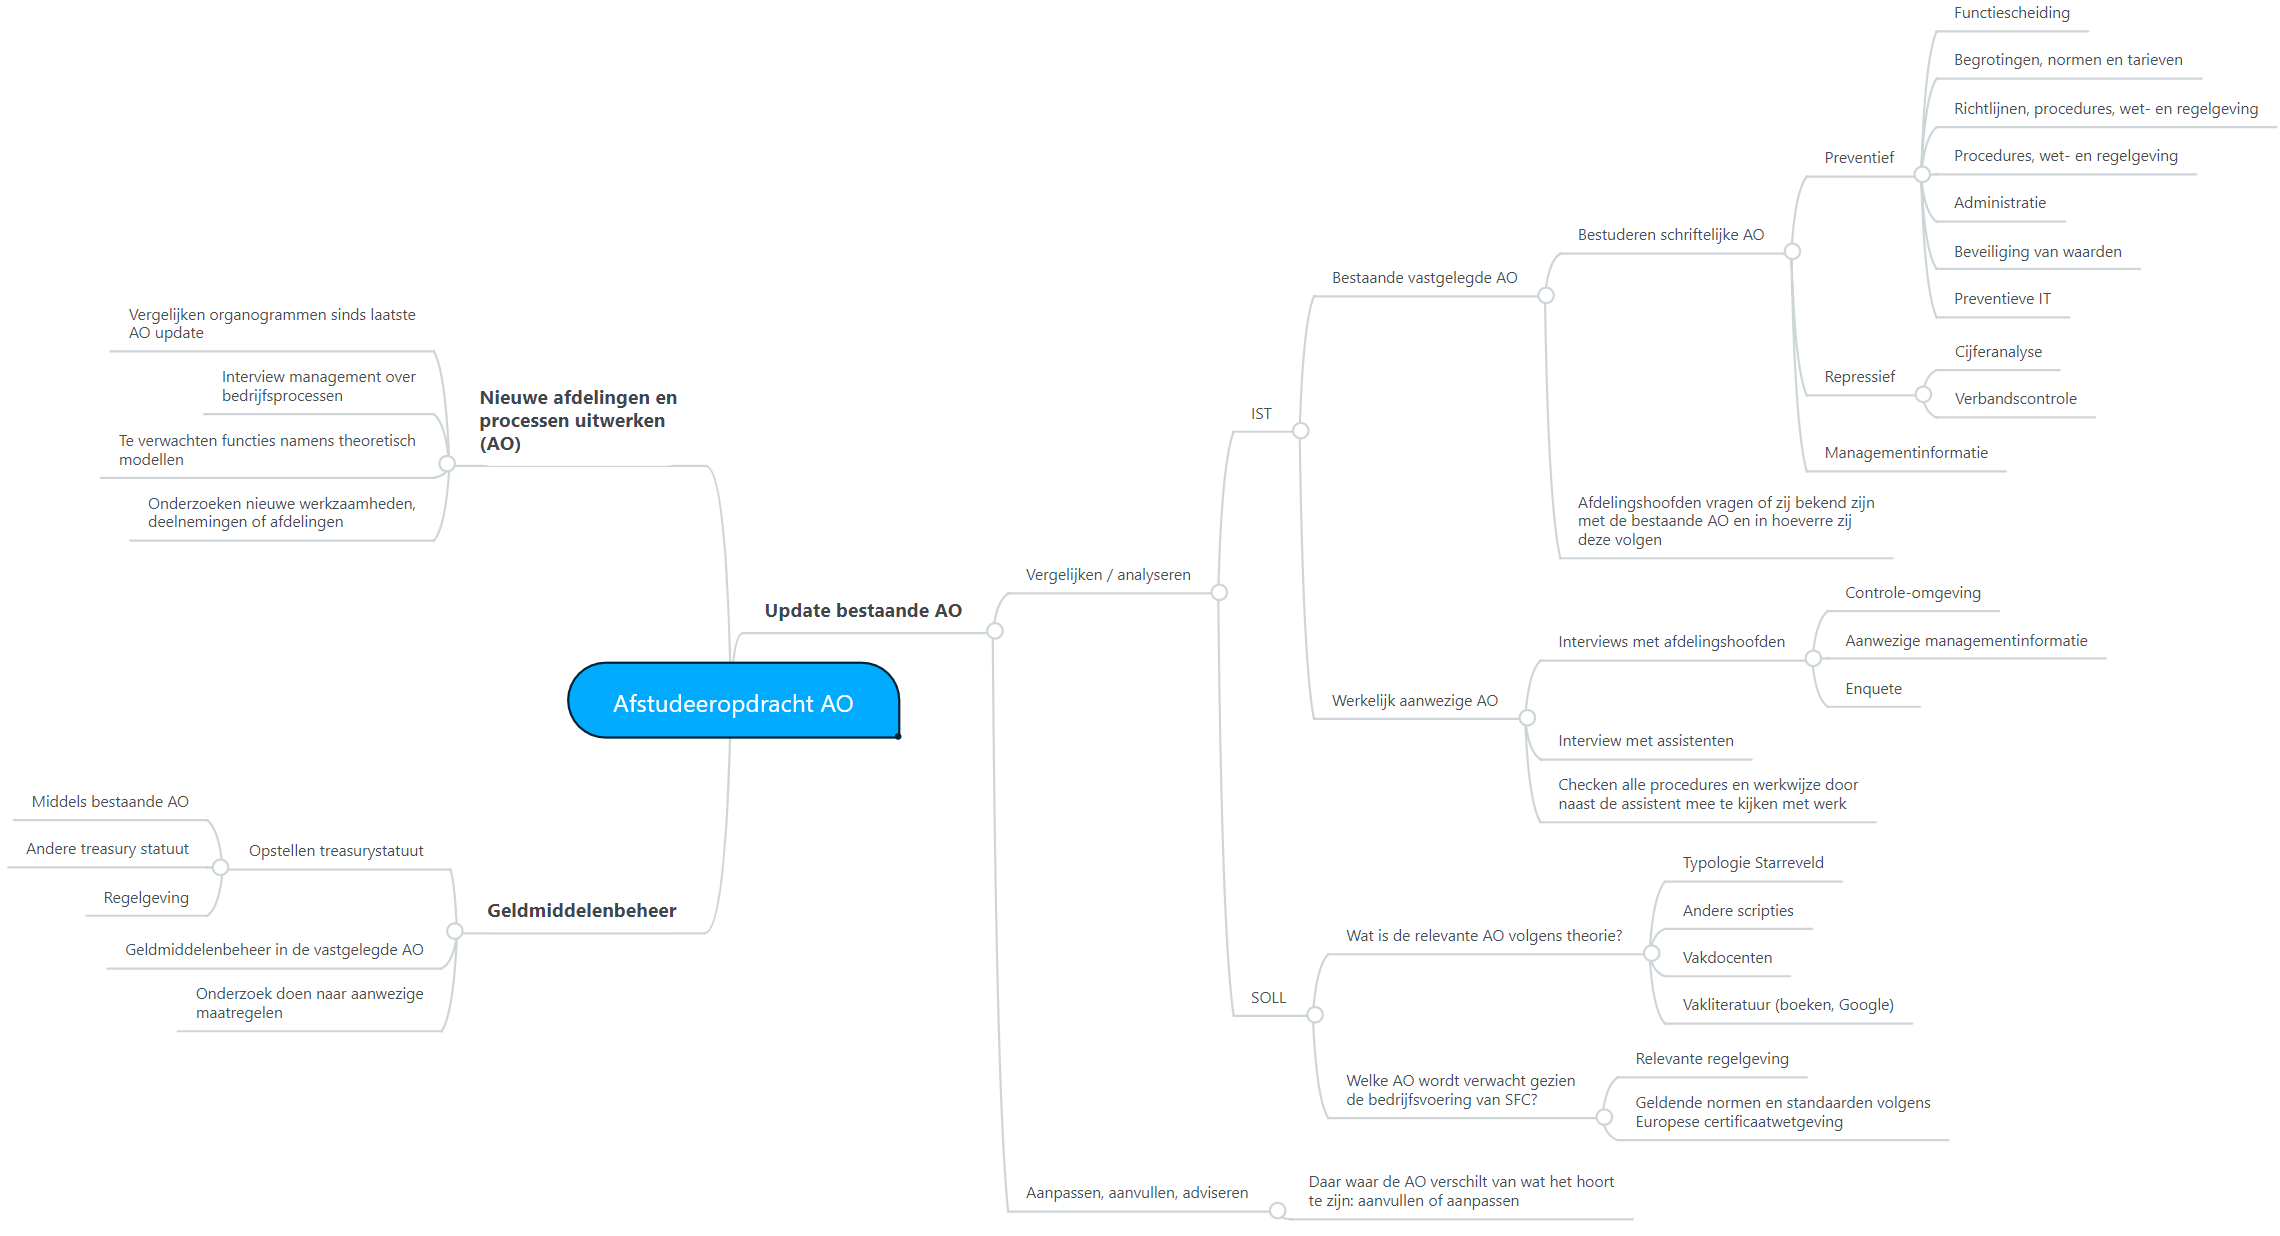
\includegraphics[angle=90,height=0.95\textheight]{afstudeeropdracht}
    \caption{Mindmap algehele afstudeeropdracht Seafood Connection}
    \label{fig:mmopdracht}
\end{figure}

\begin{figure}
    \centering
    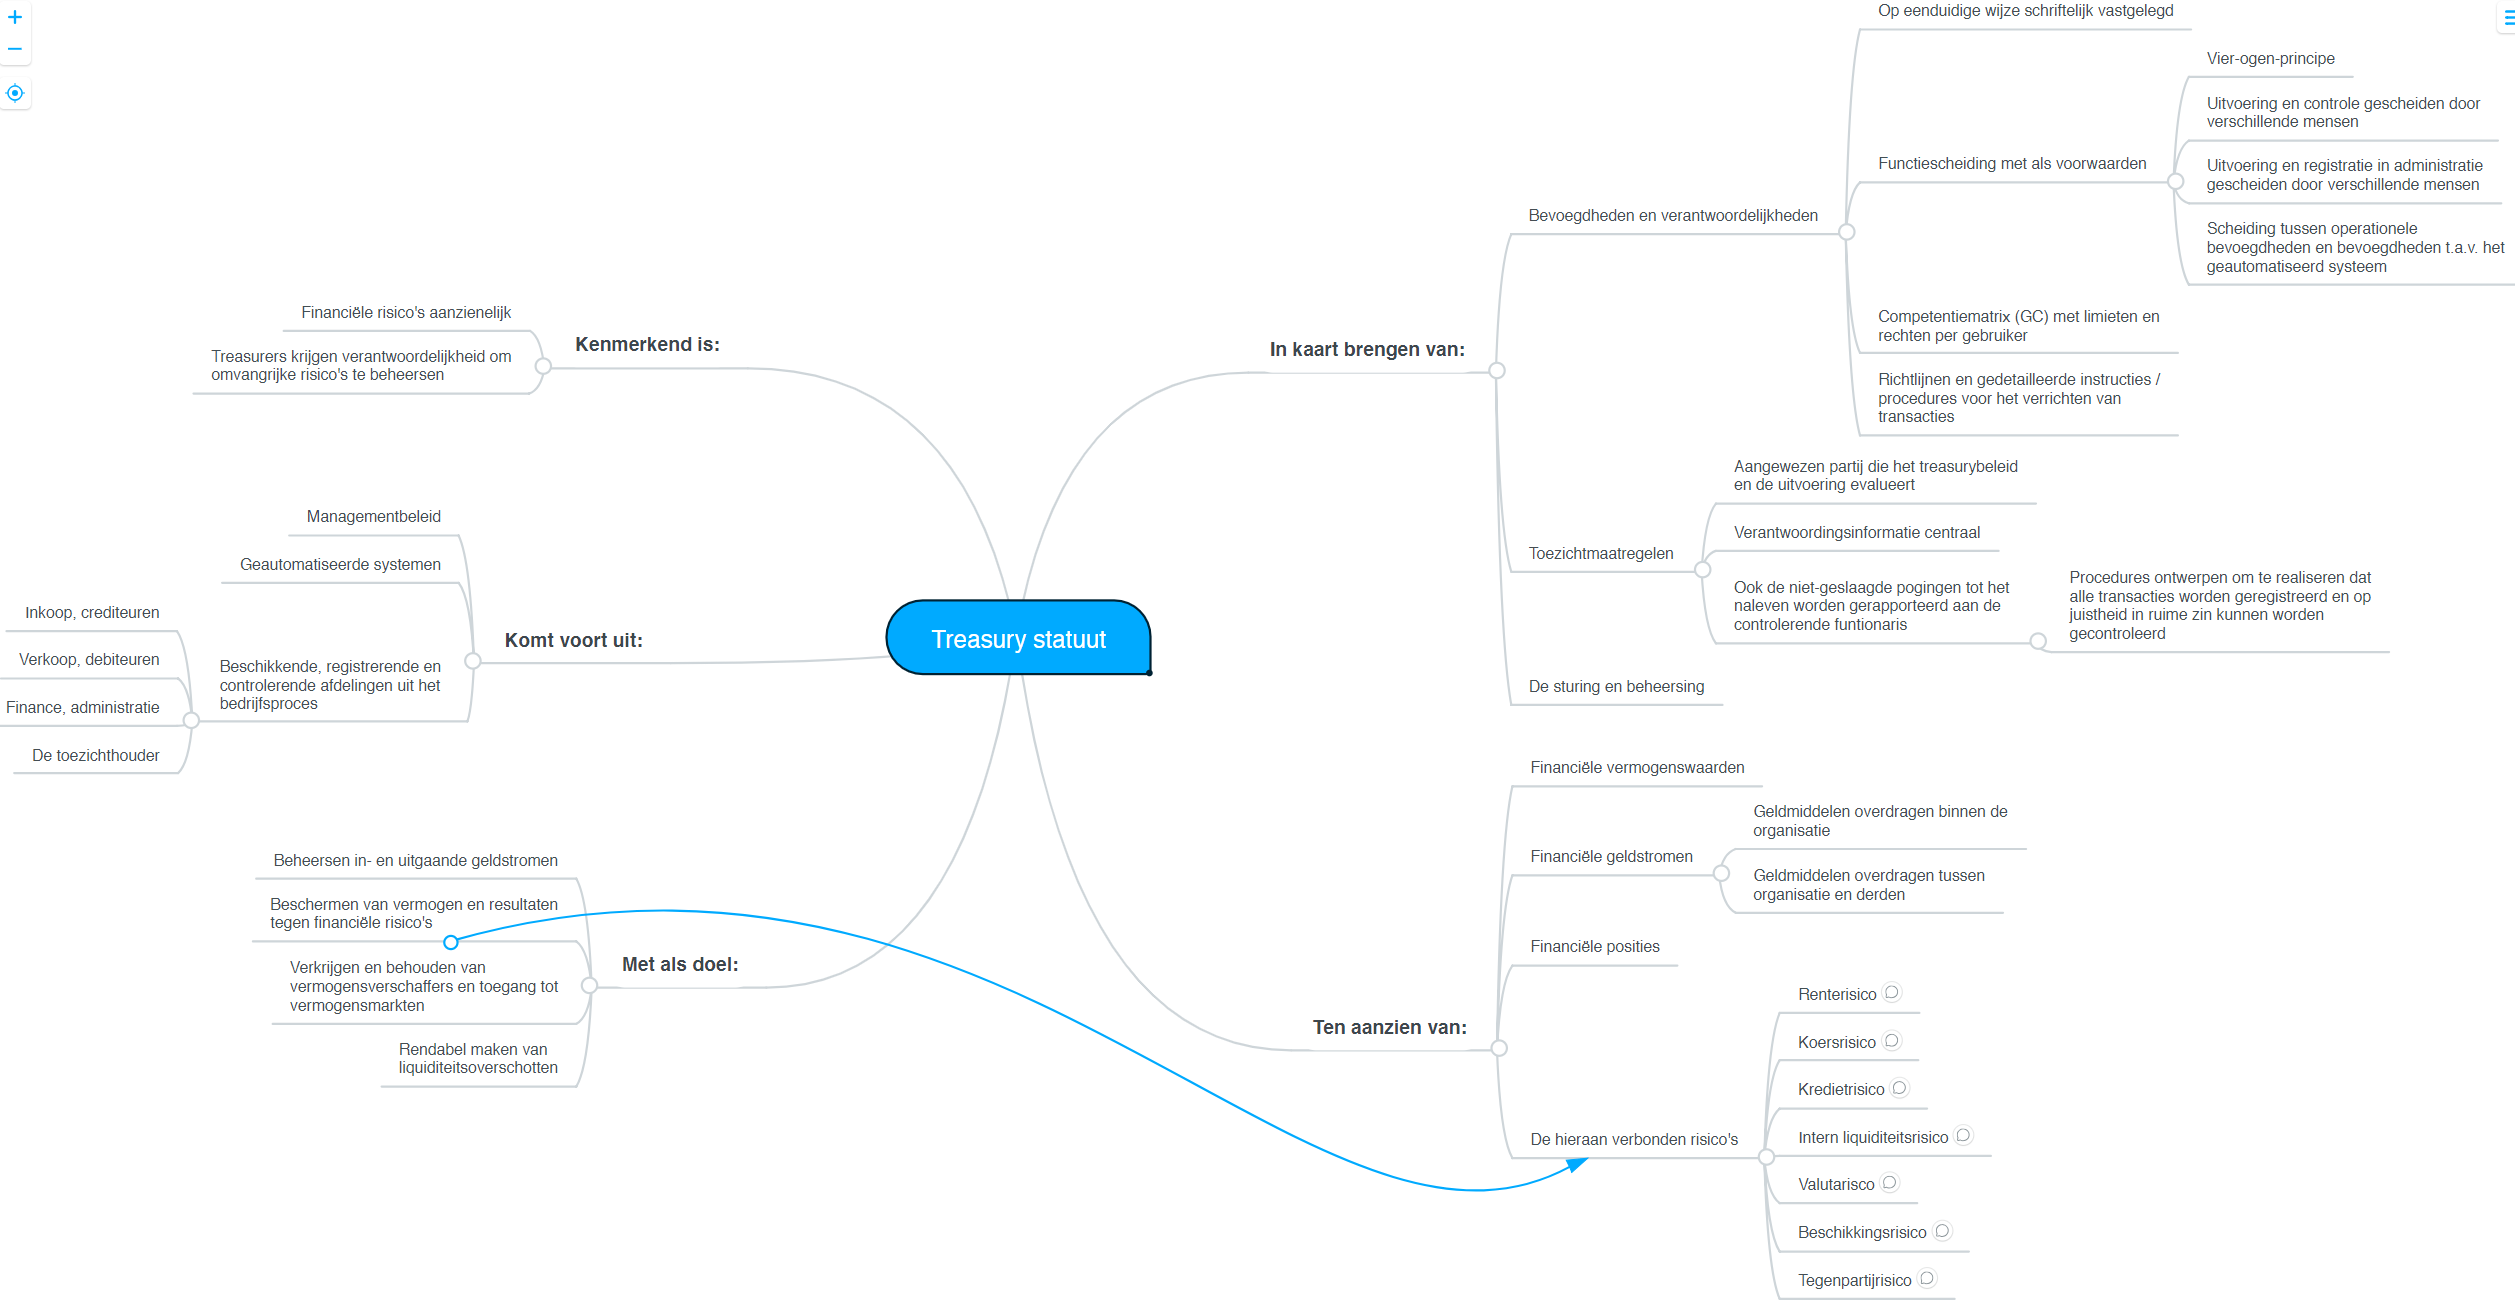
\includegraphics[angle=90,height=0.95\textheight]{treasury}
    \caption{Mindmap treasury statuut}
    \label{fig:mmtreasury}
\end{figure}
\printbibliography
\addcontentsline{toc}{chapter}{Bibliografie}
\end{document}